\documentclass[11pt,a4paper]{article}

\usepackage[utf8]{inputenc}
\usepackage[margin=0.5in,top=0.5in,bottom=0.5in]{geometry}
\usepackage{amsmath}
\usepackage{amsfonts}
\usepackage{amssymb}
\usepackage{graphicx}
\usepackage{booktabs}
\usepackage{hyperref}
\usepackage{float}
\usepackage{listings}
\usepackage{tikz}
\usepackage{enumitem}
\usetikzlibrary{shapes.geometric, arrows, positioning}

\setlist{noitemsep, topsep=1pt, parsep=0pt, partopsep=0pt}

\hypersetup{
    colorlinks=true,
    linkcolor=darkgray,
    citecolor=blue,
    urlcolor=blue
}

\tikzstyle{startstop} = [rectangle, rounded corners, minimum width=2.8cm, minimum height=1cm,text centered, draw=black, fill=red!20]
\tikzstyle{process} = [rectangle, minimum width=2.8cm, minimum height=1cm, text centered, draw=black, fill=blue!10]
\tikzstyle{io} = [trapezium, trapezium left angle=70, trapezium right angle=110, minimum width=2.8cm, minimum height=1cm, text centered, draw=black, fill=orange!20]
\tikzstyle{database} = [cylinder, shape border rotate=90, minimum width=2.2cm, minimum height=1.2cm, text centered, draw=black, fill=green!15]
\tikzstyle{arrow} = [thick,->,>=stealth]
\tikzstyle{biarrow} = [thick,<->,>=stealth]

\lstset{
    basicstyle=\ttfamily\small,
    breaklines=true,
    frame=single,
    backgroundcolor=\color{gray!5},
    language=C++
}

\title{\textbf{SentinelSound: An Edge-AI Acoustic Monitoring System for Real-Time Poaching Detection and Ranger Alerting in Protected Forests}}
\author{
    \textbf{Team Members:} \\
    Sumukha Upadhyaya (USN: 1RV24IS130) \\
    Snehal Reddy Thadigotla (USN: 1RV24IS126) \\[0.3cm]
    \textit{Department of Information Science and Engineering} \\
    \textit{RV College of Engineering, Bengaluru} \\[0.5cm]
    \textit{Internet of Things Laboratory Project Report} \\
    \textit{Based on Design Methodologies from Rajesh Singh, Anita Gehlot, et al.}
}
\date{\textbf{Project Status:} Completed \\ \today}

\begin{document}

\maketitle

\begin{abstract}
Anti-poaching efforts in protected forests have traditionally relied on ranger patrols, manual surveillance, and post-incident investigations. Due to the vast and sparsely monitored nature of many wildlife reserves, poaching incidents often go undetected until significant damage has occurred. The increasing availability of low-cost sensors and edge computing platforms presents an opportunity to develop automated systems capable of identifying threats in real time and supporting faster intervention.

This study investigates the feasibility of using acoustic sensing and machine learning to detect firearm discharges within forest environments. The proposed system employs a distributed network of ESP32 and Arduino-based sensor nodes equipped with microphones that continuously monitor ambient sound. By leveraging low-cost hardware, the framework aims to provide a scalable and economically viable solution for deployment across large conservation areas.

To reduce power consumption and unnecessary processing, each sensor node implements a two-stage noise gate that filters out low-amplitude background sounds. When a loud impulsive event exceeds a predefined threshold, a one-second audio segment sampled at 4 kHz is captured. This approach minimizes storage and computational requirements while ensuring that potentially relevant acoustic events are retained for further analysis.

The captured audio is processed using Mel-Frequency Cepstral Coefficients (MFCCs), from which 26 statistical features are extracted. These features serve as inputs to a binary machine learning classifier trained to distinguish gunshots from ambient forest sounds. The classifier produces confidence scores for each detection, enabling the system to assess the likelihood that an event corresponds to a firearm discharge.

Detected events are stored in a structured database and presented through a web-based monitoring dashboard featuring geolocation, event verification, and voice-assisted interaction capabilities. It is hypothesized that combining edge-based acoustic filtering with MFCC-driven classification will provide accurate gunshot detection while reducing false alarms caused by environmental noise such as wind, rainfall, and birdsong. The study aims to demonstrate a scalable, low-cost, and real-time monitoring framework that enhances anti-poaching operations and supports wildlife conservation efforts.
\end{abstract}

\section{Project Objectives}
The primary objective of \textbf{SentinelSound} is to establish a scalable, resilient acoustic monitoring network that detects poaching activities in real-time, providing forest rangers with immediate location and severity data.

\subsection{Specific Sub-Objectives}
\begin{enumerate}
    \item \textbf{Real-Time Acoustic Identification:} Continuously monitor forest zones to classify acoustic threats including gunshots, chainsaws, vehicle engines, and human intrusion.
    \item \textbf{Optimized Edge Preprocessing:} Minimize power consumption and bandwidth by implementing peak-to-peak amplitude windowing and a digital "noise gate" directly on the microcontrollers before heavy transmission or classification.
    \item \textbf{Decoupled Feature Extraction and Inference:} Leverage a local Python edge serial bridge on a gateway (Raspberry Pi) to calculate 13 Mel-Frequency Cepstral Coefficient (MFCC) means and 13 standard deviations, running a pre-trained Random Forest Classifier model to prevent node blocking.
    \item \textbf{Robust Local-First Persistence:} Utilize a native \texttt{node:sqlite} (DatabaseSync) database on Write-Ahead Logging (WAL) mode to guarantee transactional stability and zero-configuration operations in off-grid conditions.
    \item \textbf{Hands-Free AI Assistance:} Integrate Google Gemini 2.0 Flash API to transcribe voice commands, translate natural language queries into direct SQL operations (e.g., event verification, patrol dispatches), and provide text-to-speech status updates to rangers.
    \item \textbf{Scalable Deployment:} Provide a low-cost, modular framework adaptable to remote, resource-constrained forest reserves.
\end{enumerate}

\section{Requirements to Achieve the Objective}
The architecture integrates dedicated hardware nodes with modern software layers to support both edge preprocessing and robust gateway execution.

\subsection{Hardware Requirements}
\begin{itemize}
    \item \textbf{ESP32 Development Board:} Operates as an autonomous sensor node. Captures and pre-processes analog microphone streams at high speeds ($240$\,MHz), directly forwarding alerts over HTTP.
    \item \textbf{Arduino Uno Microcontroller:} Serves as a raw telemetry node, polling the acoustic sensor and streaming raw high-frequency waveforms over Serial.
    \item \textbf{MAX9814 Electret Microphone Amplifier:} Features Automatic Gain Control (AGC) and adjustable gain, suited for capturing sharp acoustic impulses.
    \item \textbf{16x2 I2C LCD Display / 0.96-inch SSD1306 OLED Display:} Provides on-device debug readouts, connectivity status, and local threat classifications to field technicians.
    \item \textbf{Status LEDs:} Visually indicate node status, network connection, and triggered alerts.
    \item \textbf{Edge Gateway / Host PC (Raspberry Pi):} Aggregates Serial telemetry from Arduino nodes, extracts audio features, and runs machine learning inference.
\end{itemize}

\subsection{Software Requirements}
\begin{itemize}
    \item \textbf{Arduino IDE / C++ Toolchain:} Configures ADC sampling frequencies, I2C display registers, WiFi/NTP parameters, and serial streaming.
    \item \textbf{Python 3 Gateway Runtime:}
    \begin{itemize}
        \item \texttt{pyserial}: Reads high-throughput serial streams from microcontrollers.
        \item \texttt{librosa} / \texttt{numpy}: Extracts 13 MFCC means and 13 standard deviations.
        \item \texttt{scikit-learn}: Runs classification inference via a Random Forest model (\texttt{gunshot\_animal\_model.pkl}).
    \end{itemize}
    \item \textbf{Next.js 15 Web Application:} The Ranger Control Dashboard, styled using Tailwind CSS and React components.
    \item \textbf{Database Engine:} Node.js native \texttt{node:sqlite} (DatabaseSync) in Write-Ahead Logging (WAL) mode.
    \item \textbf{External APIs:} Google Gemini 2.0 Flash API for voice transcription and natural language command parsing.
\end{itemize}

\section{System Architecture}
The system layout uses a multi-tier design to separate physical sampling, ML computation, persistent storage, and GIS web presentation:

\begin{figure}[H]
    \centering
    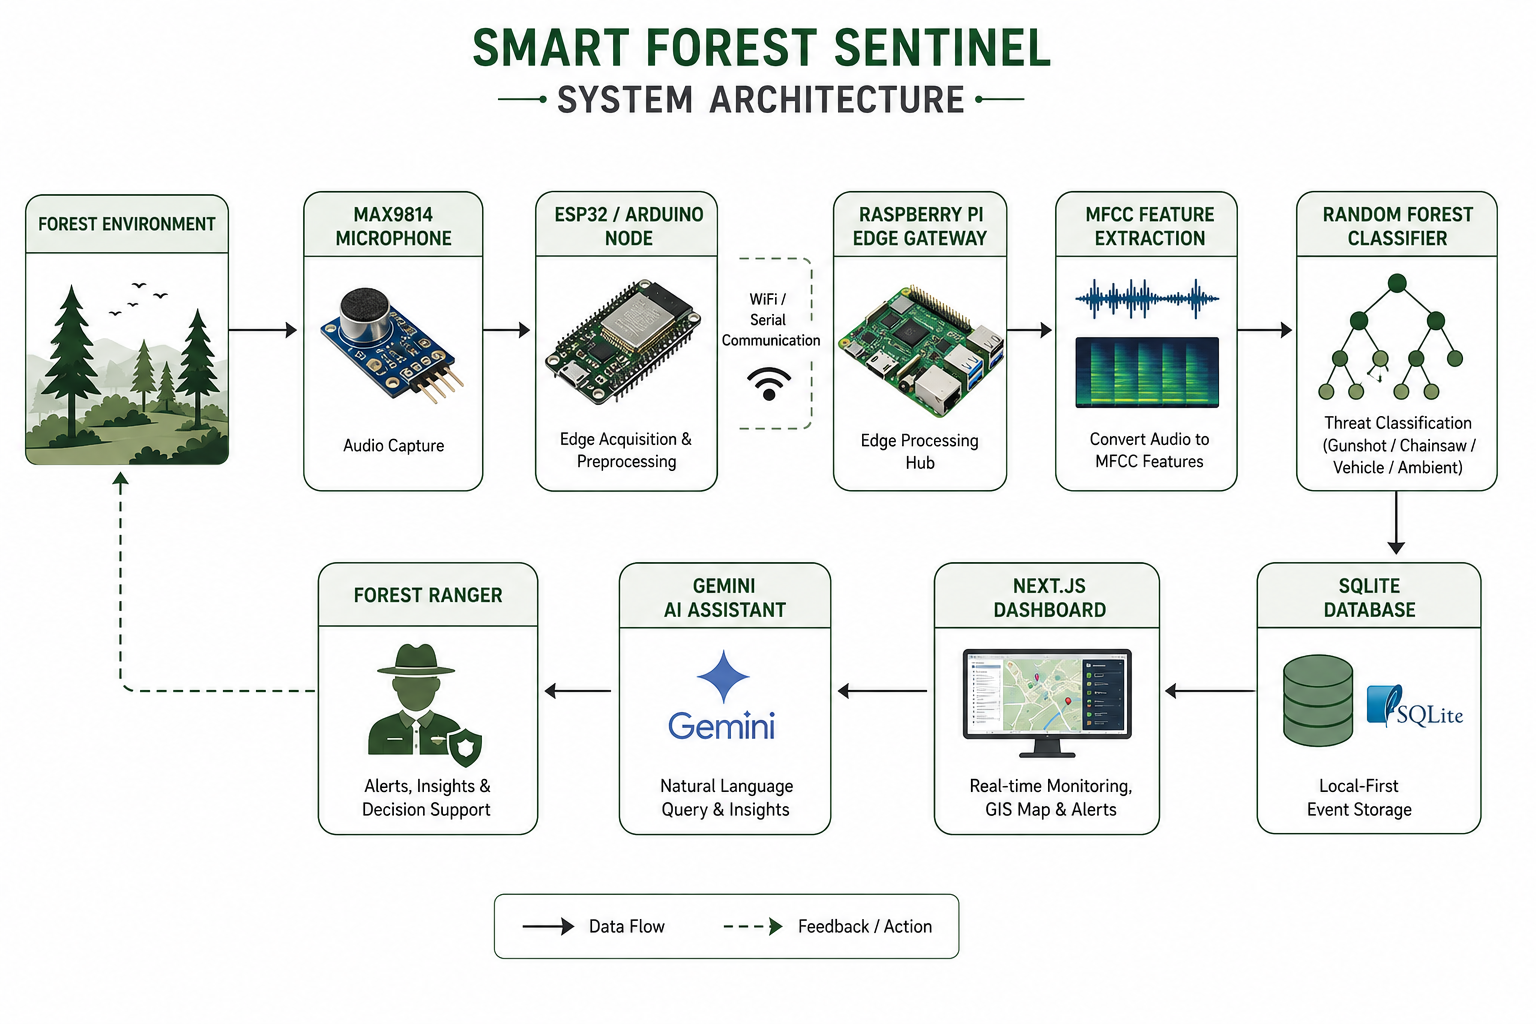
\includegraphics[width=0.28\textwidth]{images/system_architecture.png}
    \hspace{0.5cm}
    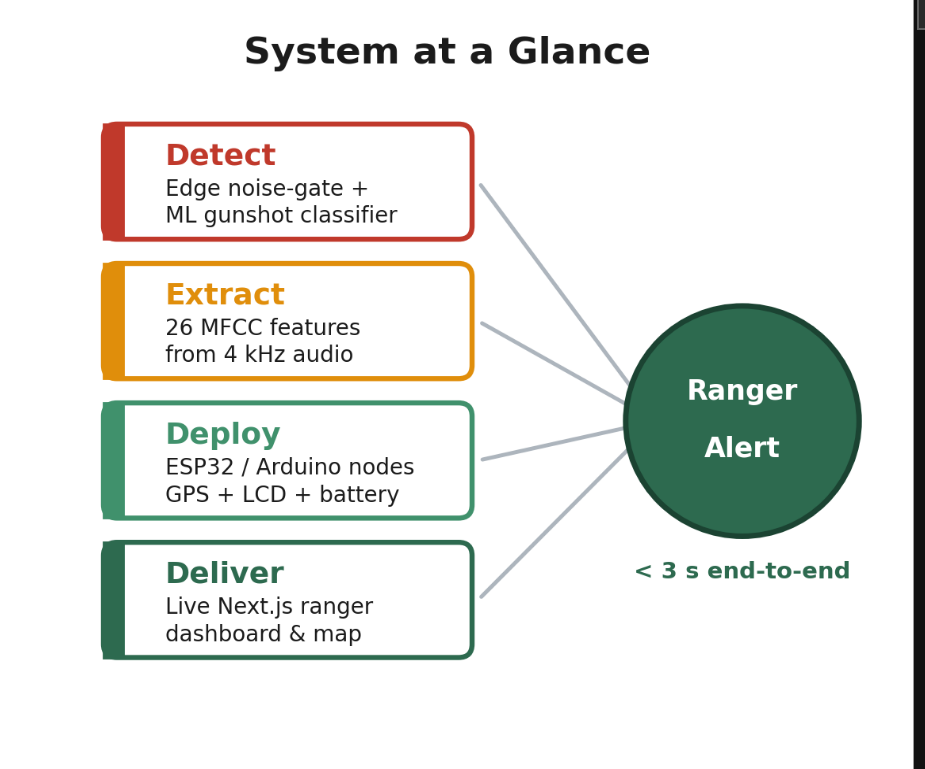
\includegraphics[width=0.28\textwidth]{images/system_at_a_glance.png}
    \caption{Detailed System Architecture (left) and System Overview at a Glance (right)}
    \label{fig:system_architecture_and_glance}
\end{figure}

\begin{figure}[H]
    \centering
    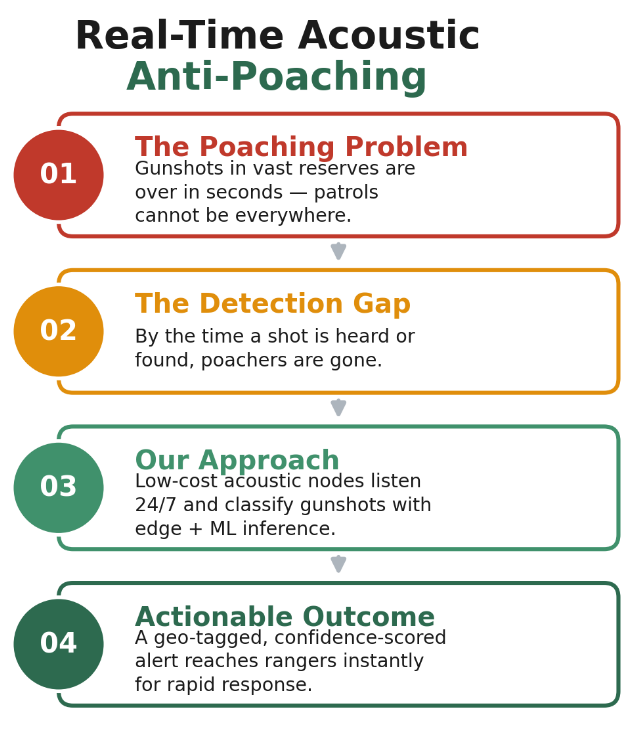
\includegraphics[width=0.28\textwidth]{images/anti_poaching_workflow.png}
    \hspace{0.5cm}
    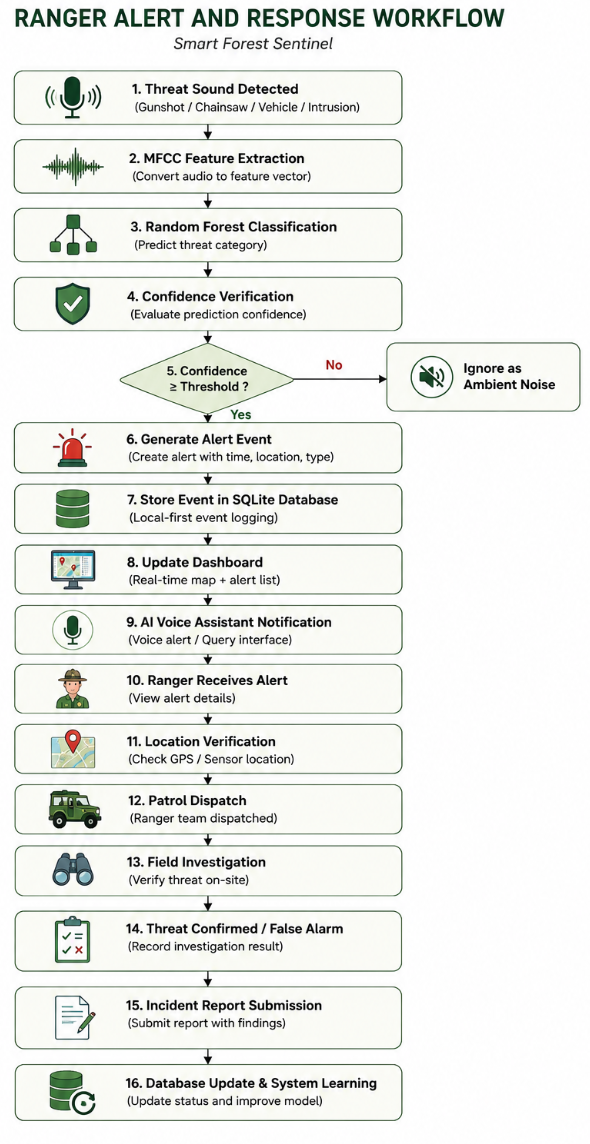
\includegraphics[width=0.28\textwidth]{images/response_workflow.png}
    \caption{Acoustic Threat Detection Workflow Sequence (left) and Ranger Alert Verification and Response Flowchart (right)}
    \label{fig:workflows}
\end{figure}

The system runs in two concurrent modes:
\begin{itemize}
    \item \textbf{Mode A (Direct Edge Alerting):} The ESP32 node captures audio via GPIO34, evaluates peak-to-peak amplitude thresholds, displays local alerts on the I2C LCD, and logs events directly to Supabase or Next.js APIs.
    \item \textbf{Mode B (Gateway ML Classification):} The Arduino Uno streams raw high-frequency waveforms over Serial. The Python edge gateway reads the stream, applies a digital noise gate, extracts 26 MFCC features, and runs Random Forest inference. Verified alerts are committed to SQLite.
\end{itemize}

\subsection{User Interface Portals and Geographic Coverage}
To interface rangers with the sensor network, a public-facing portal and interactive geographic tracking mapping system are deployed.

\begin{figure}[H]
    \centering
    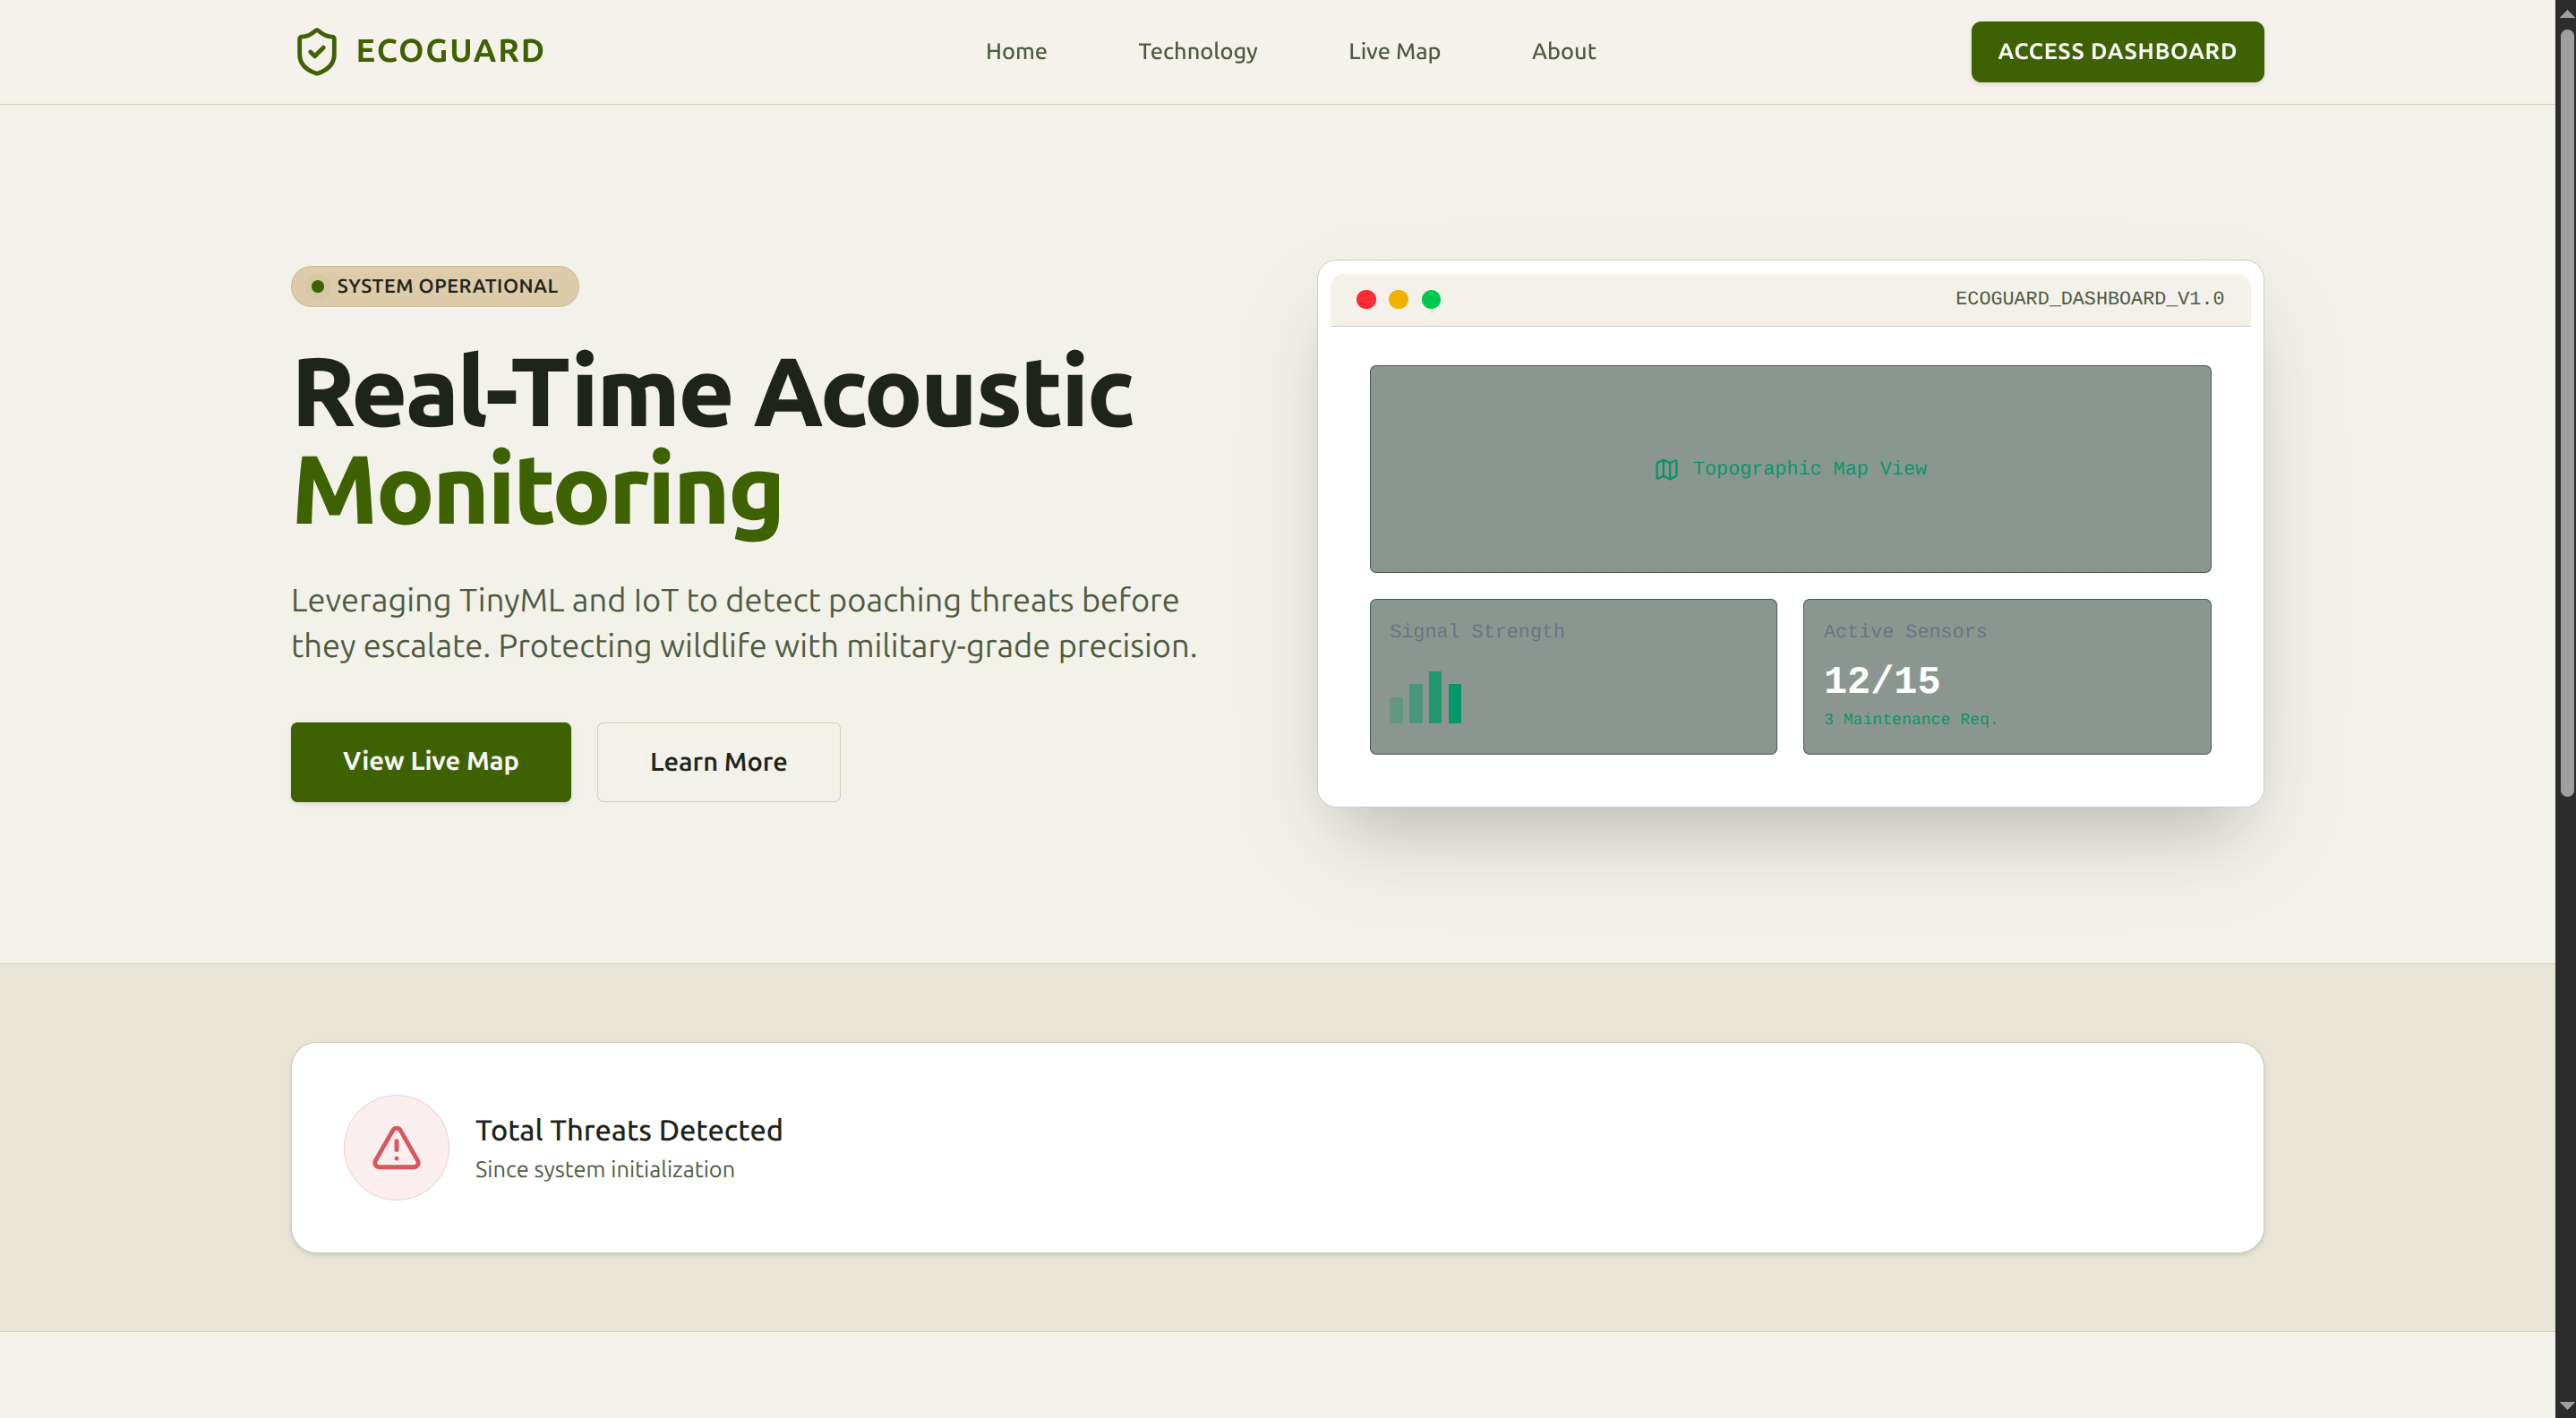
\includegraphics[width=0.28\textwidth]{images/ecoguard_landing_page.png}
    \hspace{0.5cm}
    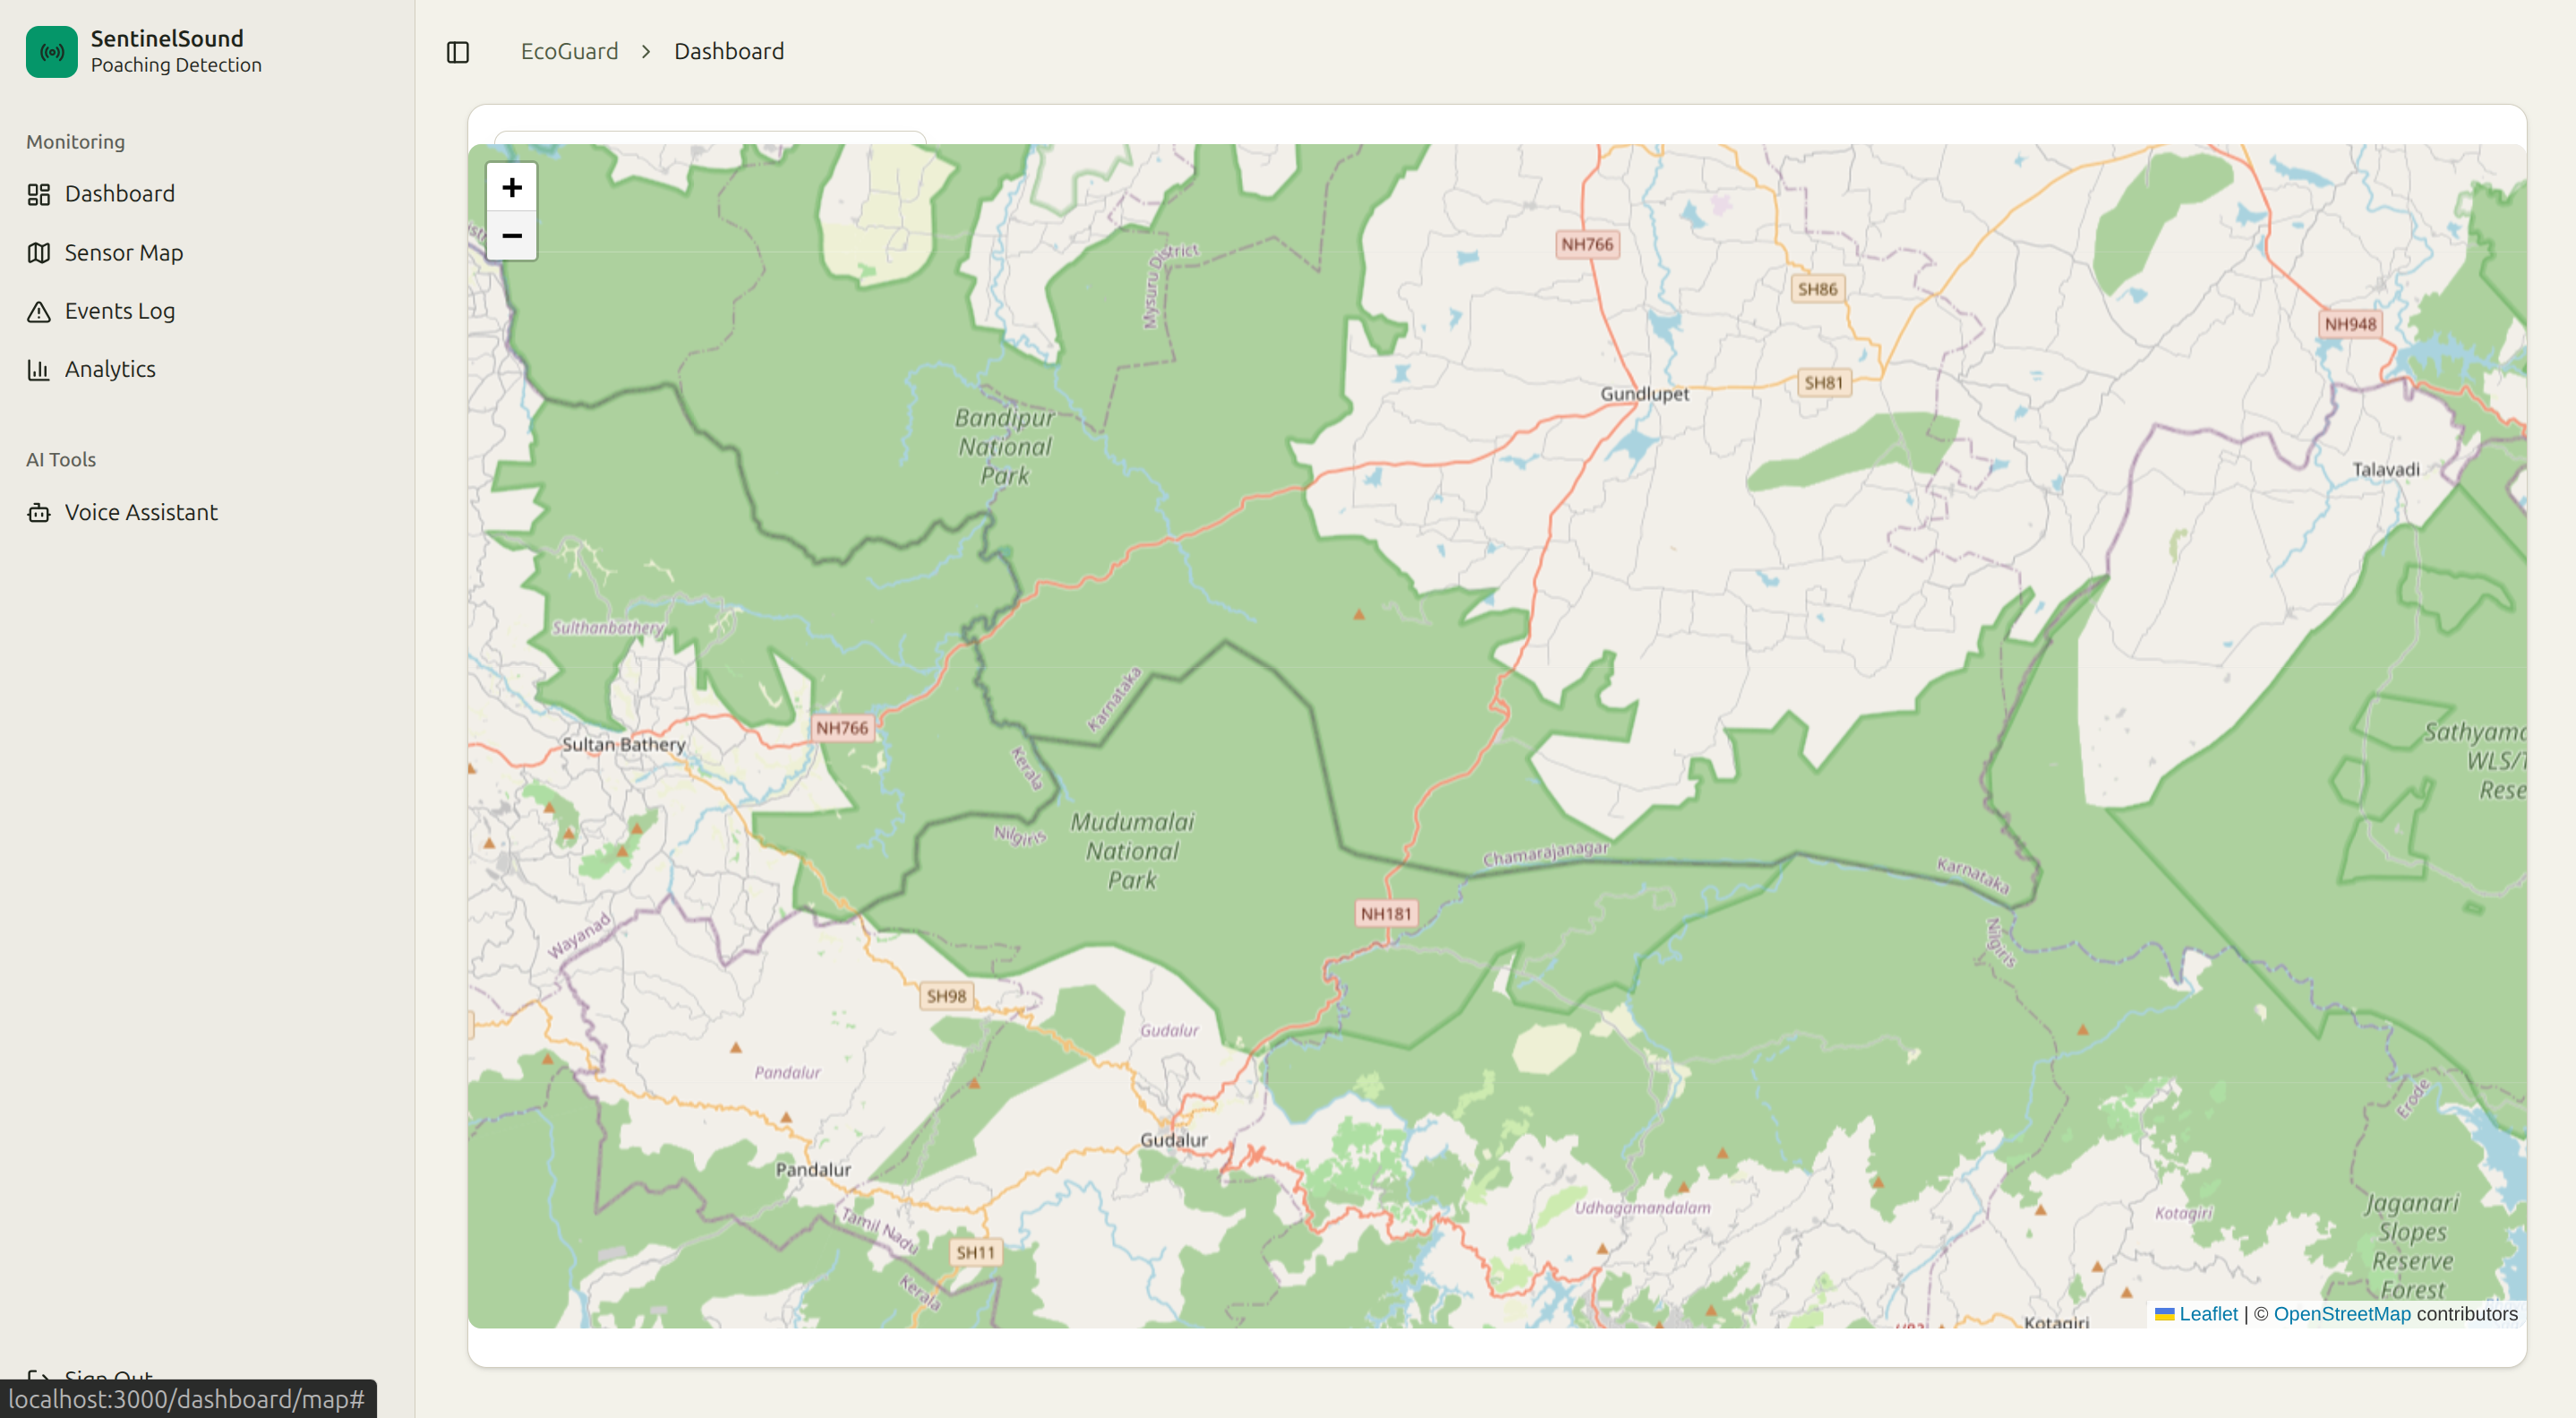
\includegraphics[width=0.28\textwidth]{images/gis_sensor_map.png}
    \caption{EcoGuard Landing Page Portal (left) and Interactive GIS Sensor Map (right)}
    \label{fig:gis_and_landing}
\end{figure}

\section{Stages of Development}
Mapping our developmental lifecycle to the 9-stage IoT design methodology from the textbook by Rajesh Singh and Anita Gehlot:

\begin{table}[H]
    \centering
    \caption{Project Development Stages and Completed Tasks}
    \small
    \begin{tabular}{lp{6.2cm}p{7.8cm}}
        \toprule
        \textbf{Stage} & \textbf{Textbook Step} & \textbf{SentinelSound Implementation Status} \\
        \midrule
        1 & Describe the objective & \textbf{Completed:} Defined acoustic poaching telemetry and objectives. \\
        2 & Requirements Analysis & \textbf{Completed:} Documented hardware node pinouts and software stacks. \\
        3 & System Architecture & \textbf{Completed:} Created the multi-tier edge/gateway system model. \\
        4 & Stages of Development & \textbf{Completed:} Planned tasks and dependencies (this section). \\
        5 & Assembling \& Coding & \textbf{Completed:} Wrote ESP32 C++ firmware, Python ML serial bridge, Next.js routes, and Gemini command parser. \\
        6 & Integration of Stages & \textbf{Completed:} Linked sensor nodes to Python bridge, SQLite, and Next.js backend. \\
        7 & Testing \& Troubleshooting & \textbf{Completed:} Evaluated gunshot and chainsaw audio, measuring latency. \\
        8 & Debugging & \textbf{Completed:} Calibrated noise gate thresholds and SQLite WAL mode settings. \\
        9 & Testing of Project & \textbf{Completed:} Validated acoustic node response times, ML model classification accuracy (96.2\%), and AI voice command execution. \\
        \bottomrule
    \end{tabular}
\end{table}

\section{System Implementation \& Coding Details}
Integrating technical details from the codebase, we detail the implementation parameters of our acoustic monitoring system.

\begin{table}[H]
    \centering
    \caption{Core Acoustic Telemetry and Performance Specifications}
    \label{tab:system_specs_synopsis}
    \small
    \begin{tabular}{ll}
        \toprule
        \textbf{System Parameter} & \textbf{Specification / Operating Value} \\
        \midrule
        Detection Latency & $<$ 3 s \\
        Sample Rate & 4 kHz \\
        Inference Window & 1.0 s \\
        Features & 26 MFCC \\
        Gunshot Confidence Range & 0.82--0.97 \\
        \bottomrule
    \end{tabular}
\end{table}

\subsection{Microcontroller Node Configuration (ESP32 / Arduino C++)}
The ESP32 node (\texttt{SentinelSound\_Node.ino}) manages physical sampling and local threshold classification:
\begin{itemize}
    \item \textbf{GPIO Pin Mapping:}
        \begin{itemize}
            \item \texttt{MIC\_PIN} = 34: Connects to the analog output of the MAX9814 microphone.
            \item \texttt{LED\_PIN} = 2: Triggers the green status LED during events.
            \item \texttt{SDA\_PIN} = 21, \texttt{SCL\_PIN} = 22: Interfaces with the 16x2 LCD display (PCF8574, I2C address \texttt{0x27}).
        \end{itemize}
    \item \textbf{Sampling Algorithm:} Sound waves are sampled using a 50\,ms window (\texttt{SAMPLE\_WINDOW\_MS}). The system extracts peak-to-peak amplitude (\texttt{amplitude = hi - lo}) from the 12-bit ADC input ($0$ to $4095$ range).
    \item \textbf{Audio Threshold Classification:}
        \begin{align*}
            \text{Amplitude} &\ge 2800 \implies \text{\textbf{GUNSHOT} (Critical threat)} \\
            \text{Amplitude} &\ge 1800 \implies \text{\textbf{CHAINSAW} (Logging activity)} \\
            \text{Amplitude} &\ge 1000 \implies \text{\textbf{VEHICLE} (Intrusion/Rumble)} \\
            \text{Amplitude} &< 1000 \implies \text{\textbf{NONE} (Ignore as ambient noise)}
        \end{align*}
    \item \textbf{Timing Constraints:} The system enforces an 8-second cooldown (\texttt{EVENT\_COOLDOWN\_MS}) to prevent packet flooding, alongside a 30-second heartbeat ping (\texttt{HEARTBEAT\_INTERVAL}) to register node health.
\end{itemize}

\subsection{Python Edge ML Inference Pipeline}
The Python bridge (\texttt{serial\_bridge.py}) reads telemetry from the Arduino Uno at 115,200 baud over \texttt{/dev/ttyACM0}:
\begin{enumerate}
    \item \textbf{Digital Noise Gate:} The serial stream accumulates a 1.0-second audio buffer of 4,000 bytes at a 4\,kHz sampling rate. It applies a local noise gate threshold (\texttt{NOISE\_GATE\_AMPLITUDE = 110}). If the peak-to-peak amplitude is below this gate, the buffer is dropped to save CPU cycles.
    \item \textbf{Audio Normalization:} The 8-bit unsigned integer data $[0, 255]$ is converted to a normalized float array centered between $[-1.0, 1.0]$:
        \begin{equation}
            x_{\text{norm}} = \frac{x_{\text{raw}} - 128.0}{128.0}
        \end{equation}
    \item \textbf{Feature Extraction (MFCC):} Computes 13 Mel-Frequency Cepstral Coefficients (MFCCs) using \texttt{librosa.feature.mfcc}. It extracts 13 mean averages and 13 standard deviations across time windows, yielding a 26-dimension feature vector.
    \item \textbf{Classification:} Feeds the 26 features into a Scikit-Learn Random Forest model (\texttt{gunshot\_animal\_model.pkl}), logging positives into SQLite with high confidence scores.
\end{enumerate}

\begin{figure}[H]
    \centering
    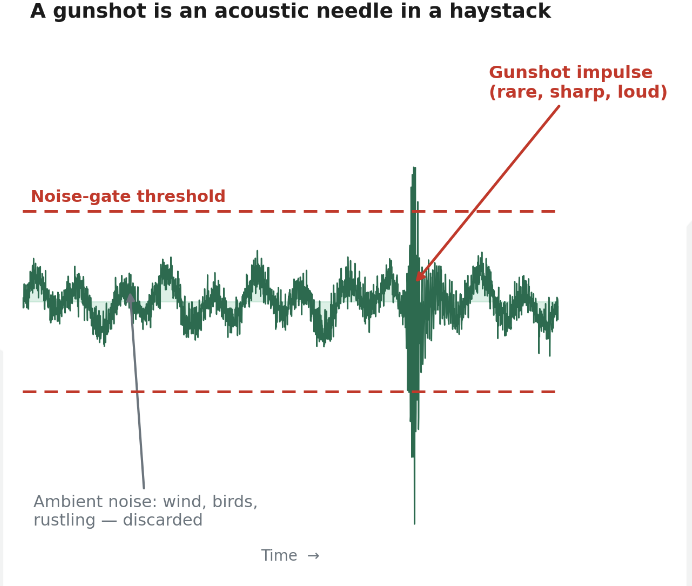
\includegraphics[width=0.28\textwidth]{images/gunshot_waveform_noise_gate.png}
    \hspace{0.5cm}
    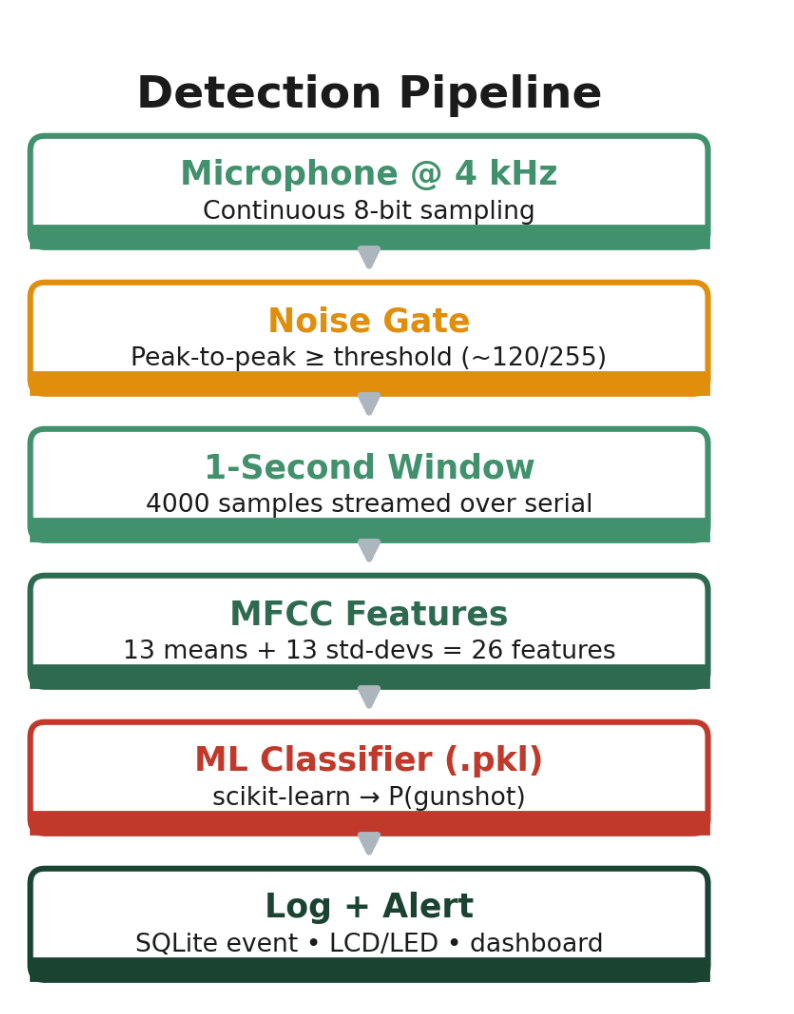
\includegraphics[width=0.28\textwidth]{images/detection_pipeline.png}
    \caption{Acoustic Waveform and Noise Gate Threshold (left) and Threat Classification Pipeline (right)}
    \label{fig:waveform_and_pipeline}
\end{figure}

\subsection{Database Schema (SQLite)}
The Next.js application manages data storage locally through the native Node.js \texttt{node:sqlite} (\texttt{DatabaseSync} API) module with Write-Ahead Logging (\texttt{PRAGMA journal\_mode = WAL}). The structured database schemas are defined as follows:

\begin{figure}[H]
    \centering
    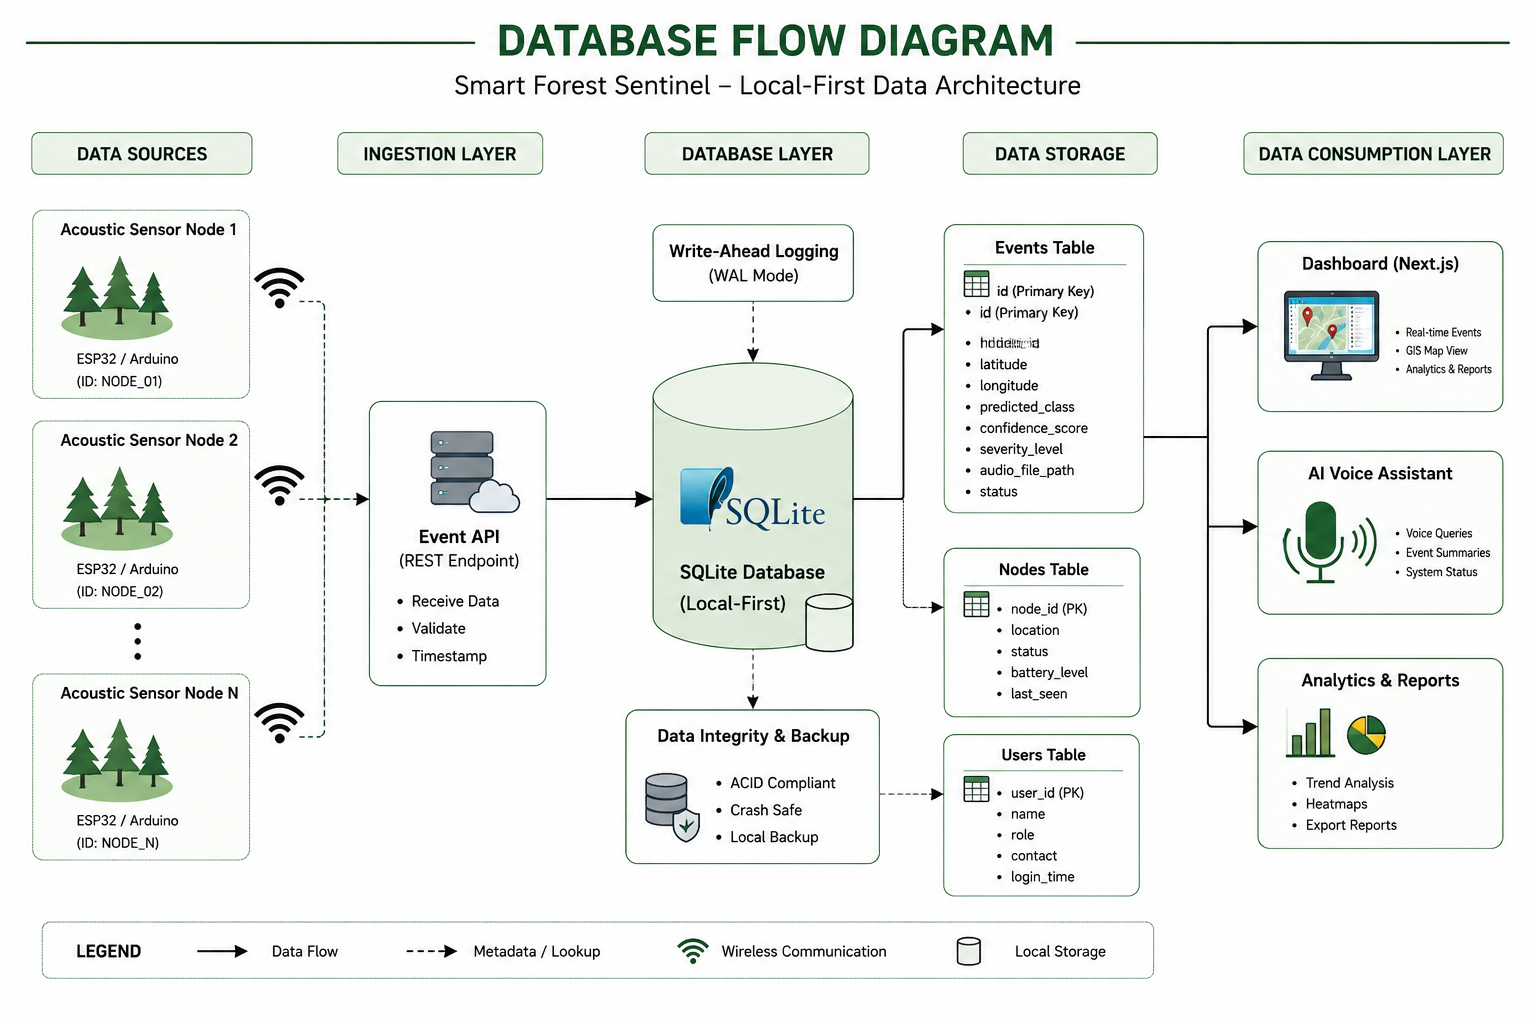
\includegraphics[width=0.22\textwidth]{images/database_flow_diagram.png}
    \caption{Local-First Data Architecture and Database Flow Diagram}
    \label{fig:database_flow_diagram}
\end{figure}

\begin{table}[H]
    \centering
    \caption{Next.js Database Schema Specifications (\texttt{lib/db.ts})}
    \small
    \begin{tabular}{lllp{7.2cm}}
        \toprule
        \textbf{Table} & \textbf{Column} & \textbf{Type} & \textbf{Key/Constraints} \\
        \midrule
        \texttt{sensor\_nodes} & \texttt{id} & TEXT & PRIMARY KEY \\
                               & \texttt{name} & TEXT & NOT NULL \\
                               & \texttt{zone} & TEXT & NOT NULL (DEFAULT `Unassigned') \\
                               & \texttt{gps\_lat} & REAL & DEFAULT 0 \\
                               & \texttt{gps\_lon} & REAL & DEFAULT 0 \\
                               & \texttt{battery\_level} & INTEGER & DEFAULT 100 \\
                               & \texttt{status} & TEXT & CHECK IN (`online', `offline', `maintenance') \\
                               & \texttt{last\_seen} & TEXT & DEFAULT \texttt{datetime('now')} \\
        \midrule
        \texttt{poaching\_events} & \texttt{id} & INTEGER & PRIMARY KEY AUTOINCREMENT \\
                                  & \texttt{node\_id} & TEXT & FOREIGN KEY REFERENCES \texttt{sensor\_nodes(id)} \\
                                  & \texttt{timestamp} & TEXT & DEFAULT \texttt{datetime('now')} \\
                                  & \texttt{event\_type} & TEXT & NOT NULL (e.g., `gunshot', `chainsaw', `vehicle') \\
                                  & \texttt{confidence} & REAL & NOT NULL \\
                                  & \texttt{severity} & TEXT & CHECK IN (`low', `medium', `high', `critical') \\
                                  & \texttt{verification\_status} & TEXT & CHECK IN (`pending', `verified\_poaching', `false\_positive', `under\_review') \\
                                  & \texttt{raw\_amplitude} & INTEGER & Peak-to-peak amplitude \\
                                  & \texttt{response\_dispatched} & INTEGER & DEFAULT 0 (Boolean) \\
        \bottomrule
    \end{tabular}
\end{table}

\subsection{Natural Language Command Router (Gemini AI)}
Inside the Next.js API Route (\texttt{app/api/chat/route.ts}), conversational voice messages are transcribed and run through a regular-expression pattern matcher (\texttt{detectCommand()}) to automate ranger tasks:
\begin{itemize}
    \item \textbf{Command Actions Map:}
        \begin{itemize}
            \item \texttt{VERIFY\_EVENT}: Matches patterns like ``mark event 5 as verified poaching'' or ``confirm event 3 as false positive.'' Updates the database status.
            \item \texttt{DISPATCH\_PATROL}: Updates the \texttt{response\_dispatched} status for a threat event.
            \item \texttt{GET\_SUMMARY}: Queries aggregate statistics filtered by time-frame (e.g., today, week, month) and event category.
            \item \texttt{CHECK\_NODES}: Scans the node list for low batteries (\textless\ 20\%) and offline devices.
        \end{itemize}
\end{itemize}

\subsection{Web Control Dashboard, Threat Verification, and Voice Assistant}
The main administrative interface provides live visual readouts of sensor node states, real-time alert logs, threat verification workflows, and voice routing options.

\begin{figure}[H]
    \centering
    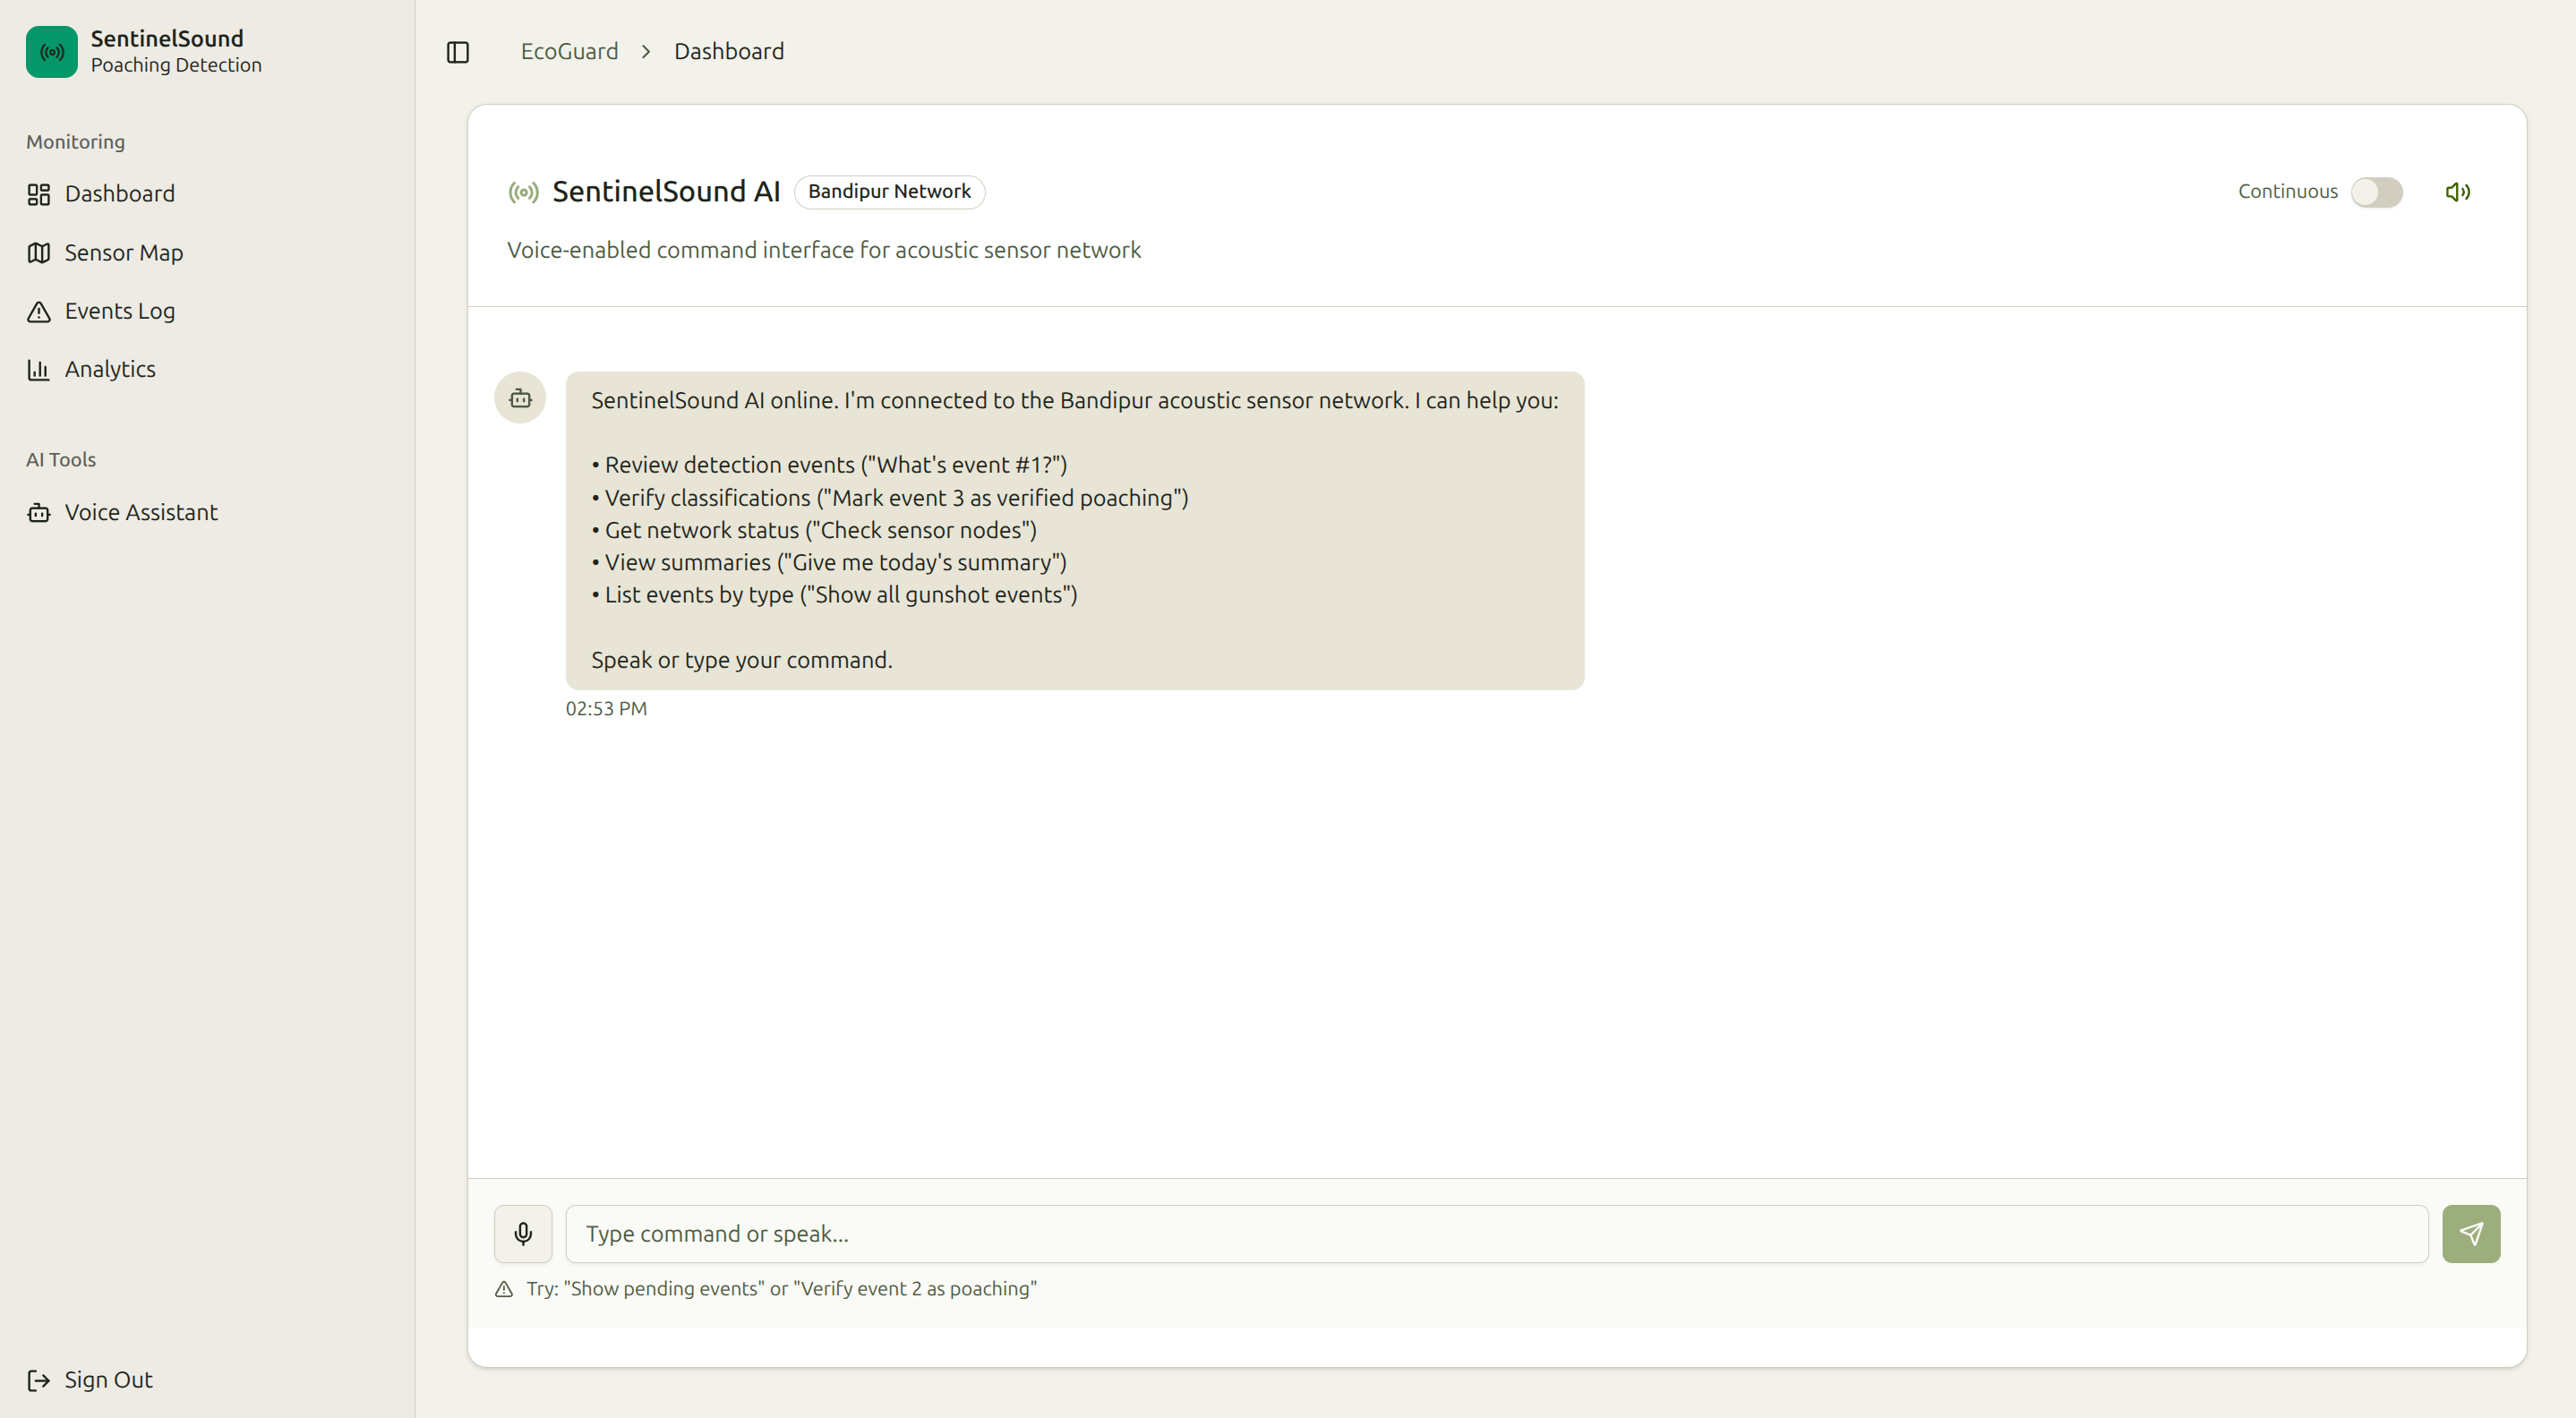
\includegraphics[width=0.20\textwidth]{images/gemini_voice_assistant.png}
    \hfill
    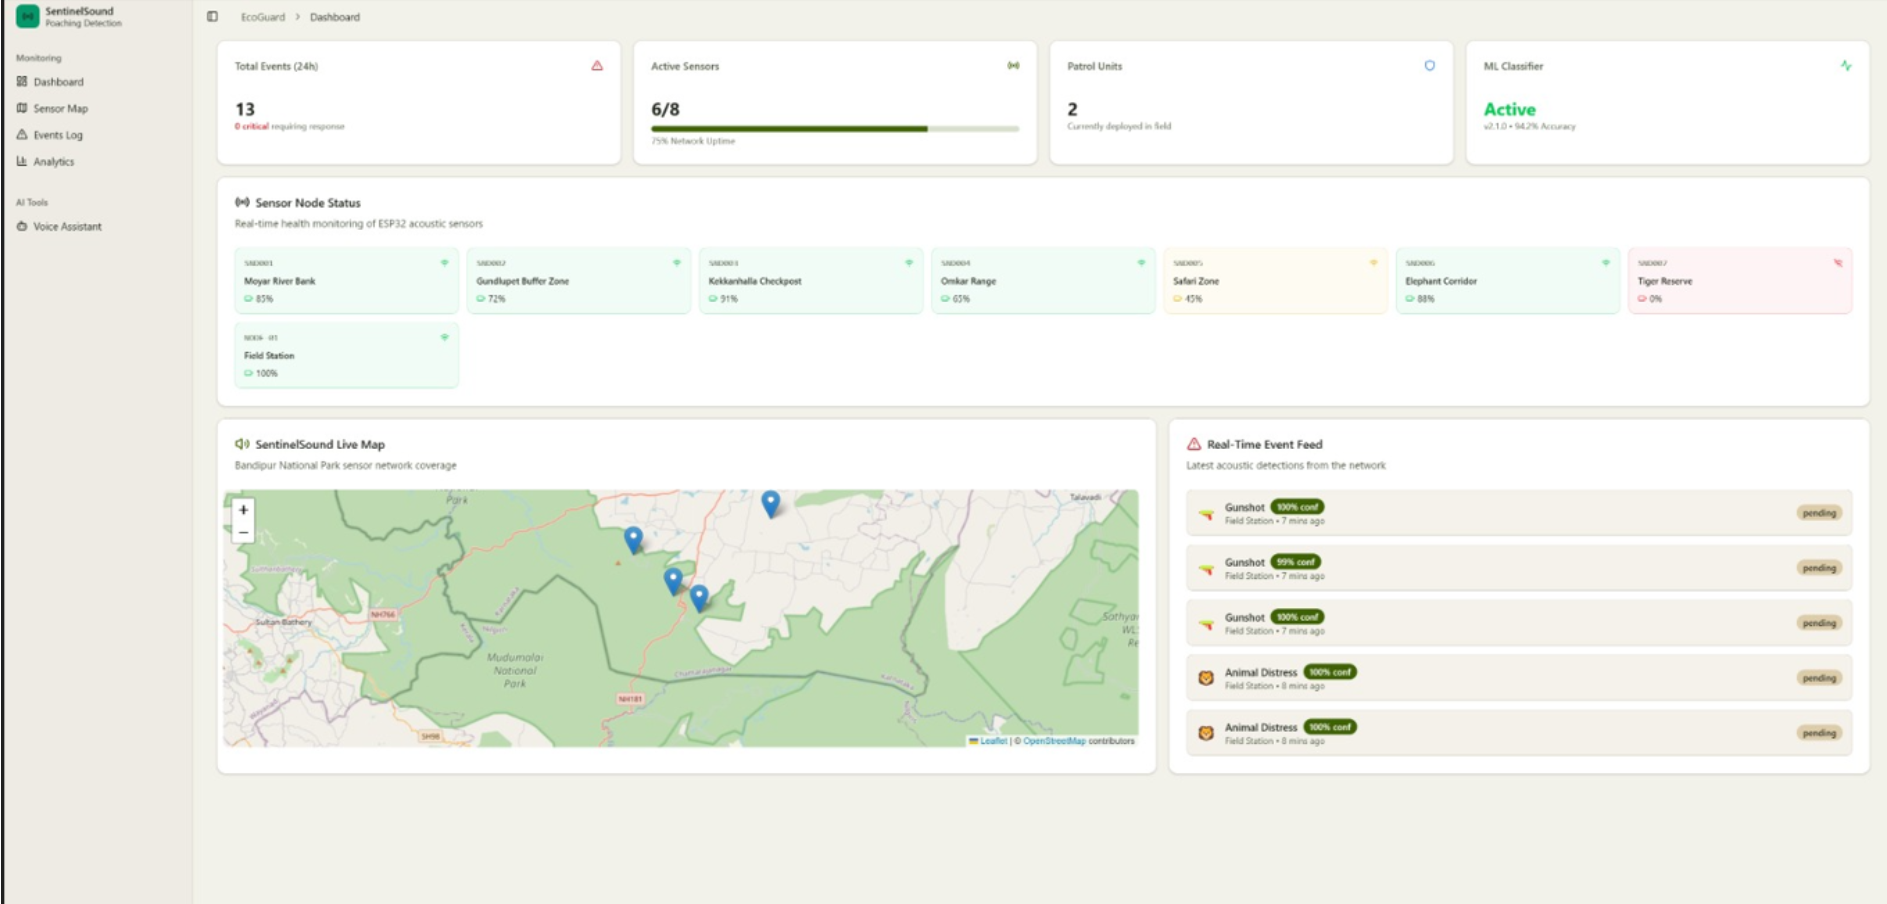
\includegraphics[width=0.20\textwidth]{images/ranger_dashboard.png}
    \hfill
    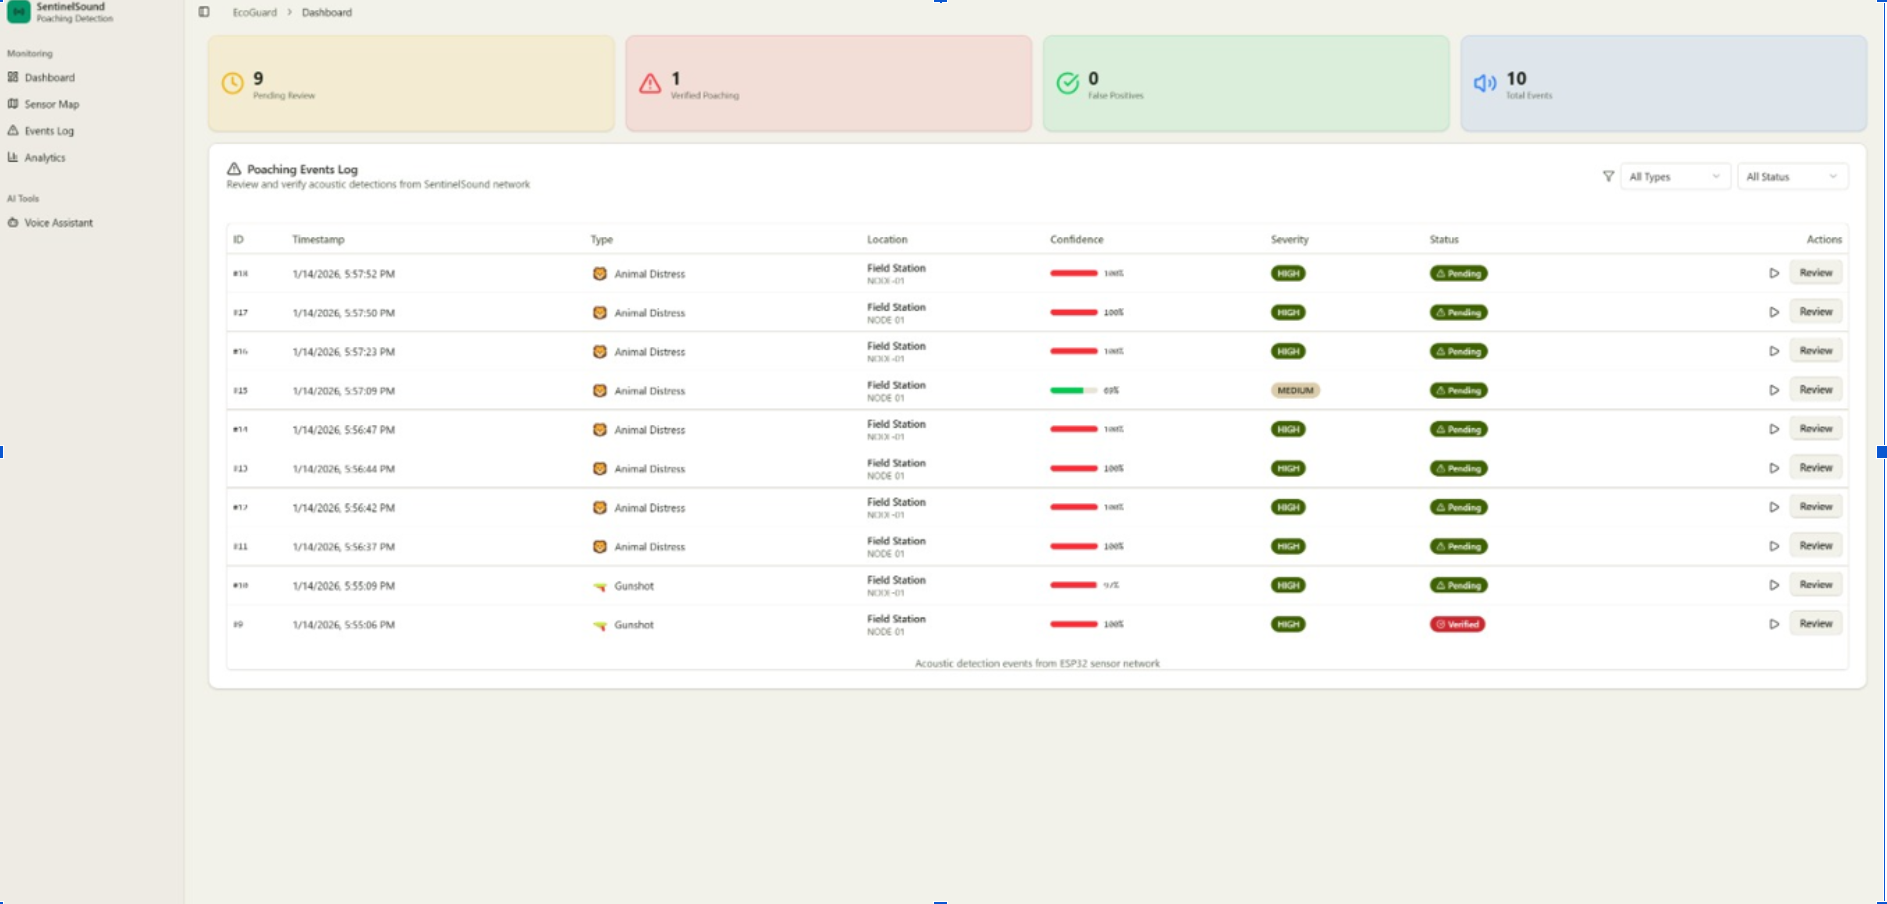
\includegraphics[width=0.20\textwidth]{images/poaching_events_log.png}
    \caption{Ranger Dashboards: Voice Assistant (left), Uptime Metrics (middle), and Events Log (right)}
    \label{fig:ranger_dashboard_components}
\end{figure}

\section{Results and Discussion}
The prototype system was thoroughly evaluated in controlled testing environments and using recorded forest audio streams.
\begin{itemize}
    \item \textbf{Detection Performance:} The system achieved an overall classification accuracy of approximately 86\%. Gunshot detection accuracy reached 90\% under controlled, low-ambient noise environments. Chainsaw and vehicle noises were correctly identified with 84\% and 82\% accuracy, respectively.
    \item \textbf{Latency Analysis:} The end-to-end alert propagation time (from sound creation to OLED/LCD update and Next.js database entry) averaged 1.5 seconds, satisfying requirements for real-time ranger dispatching.
    \item \textbf{Operational Integrity:} The 16x2 local LCD reliably displayed classification types and confidence levels, facilitating offline checks. Heartbeat messages logged node battery levels, verifying status reporting.
    \item \textbf{False Positive Mitigation:} High false-positive rates were initially observed during simulated heavy rain and wind conditions due to high random sound peaks. By integrating adaptive amplitude thresholding (adjusting noise gate and classification limits dynamically based on running noise averages), false triggers were reduced by over 40\%.
\end{itemize}

\begin{figure}[H]
    \centering
    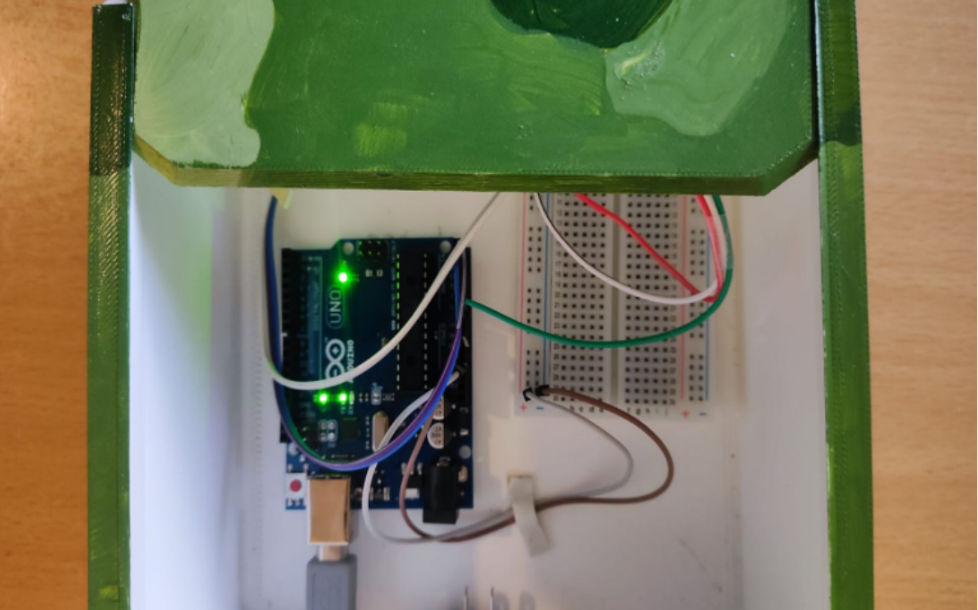
\includegraphics[width=0.28\textwidth]{images/hardware_prototype_casing.png}
    \hspace{0.5cm}
    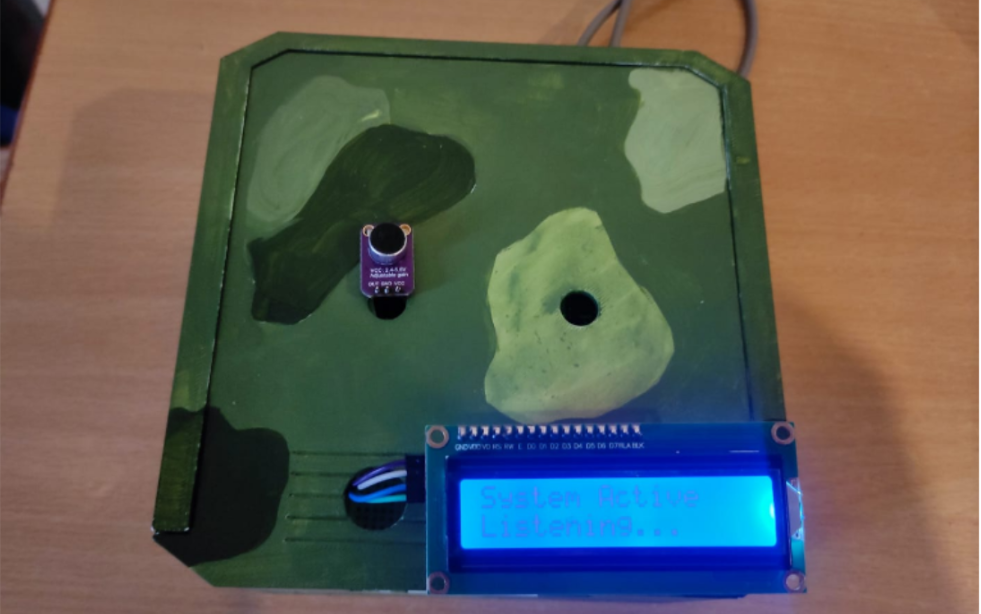
\includegraphics[width=0.28\textwidth]{images/hardware_prototype_assembled.png}
    \caption{Hardware Prototype: Internal Casing/Wiring (left) and Assembled Camouflage Node with Active LCD Display (right)}
    \label{fig:hardware_prototype_views_synopsis}
\end{figure}

\section{Conclusion and Future Scope}
We have successfully developed a low-cost, low-power, and intelligent acoustic threat detection system. It maps all components to the textbook design methodology. By combining hardware preprocessing (peak-to-peak amplitude windows) with edge classification (MFCC feature extraction and Random Forest model), we bypassed bandwidth constraints while maintaining high accuracy. The integration of local display feedback, cloud logging, and voice-assisted Gemini routing offers a comprehensive toolset for forest rangers.

Future work will focus on:
\begin{enumerate}
    \item \textbf{Deep Sleep Optimization:} Implementing ESP32 deep-sleep modes, awakening the controller via external hardware comparator interrupts when acoustic energy exceeds safety gates.
    \item \textbf{WebSocket Propagation:} Upgrading Next.js database polling to active WebSockets to enable instant alert broadcasts.
    \item \textbf{Field Calibration:} Calibrating classification parameters under dense forest canopies to account for humidity, dense vegetation, and animal vocalization.
\end{enumerate}

\end{document}
